%!TEX root = ../../report.tex
\section{Test of positioning}
\label{test}
In order to test whether the positioning system calculates the correct position two test are conducted.
In each test a ball is dropped on to the same position of the base plate multiple times.

\begin{figure}[htb]
	\centering
	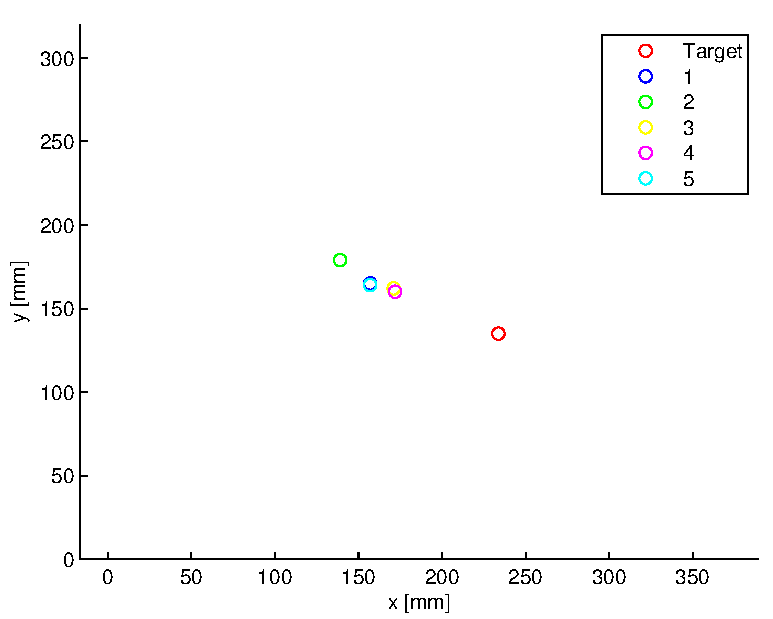
\includegraphics[width=.8\textwidth]{figures/testRes30deg.pdf}
	\caption{Estimated impact positions based as a result of dropping a ball on to the same target multiple times.}
	\label{fig:testRes30deg}
\end{figure}

\begin{figure}[htb]
	\centering
	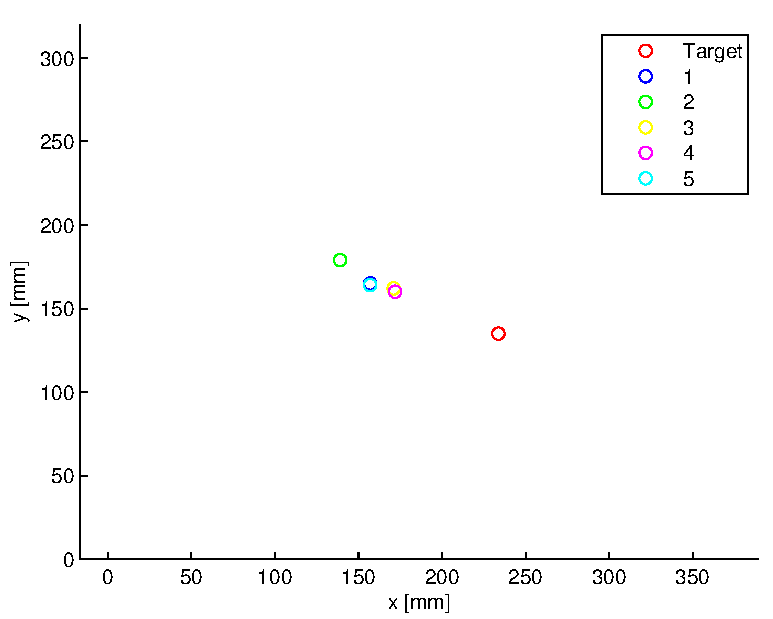
\includegraphics[width=.8\textwidth]{figures/testRes15deg.pdf}
	\caption{Estimated impact positions based as a result of dropping a ball on to the same target multiple times.}
	\label{fig:testRes15deg}
\end{figure}
